\section{Interface Iteration}\label{interface-iteration}

\begin{quote}
\begin{quote}
TODO: figure showing alpha UI
\end{quote}
\end{quote}

discuss move from drawing cuts \& folds directly to templating

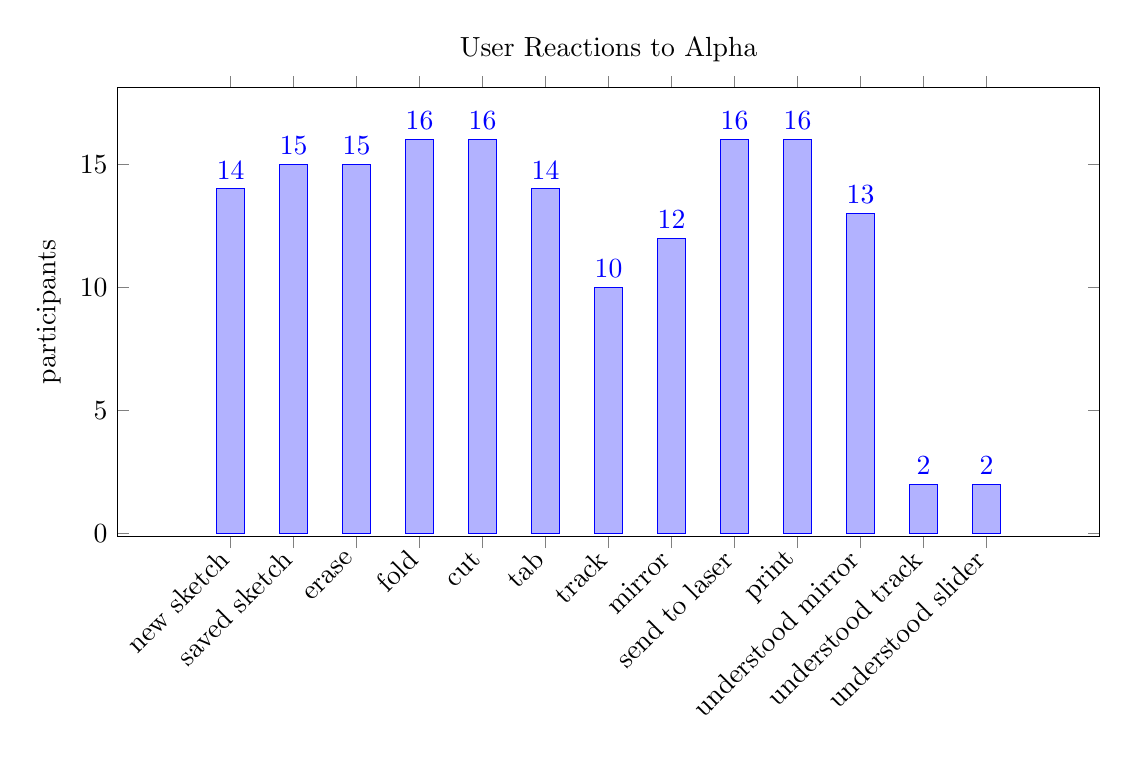
\begin{tikzpicture}
  \begin{axis}[
    title=User Reactions to Alpha,
    ybar,
    enlargelimits=0.15,
    x=0.8cm,
    legend style={at={(0.5,-0.2)},
      anchor=north,legend columns=-1},
    ylabel={participants},
    symbolic x coords={new sketch,saved sketch,erase,fold,cut,tab,track,mirror,send to laser,print,understood mirror,understood track,understood slider},
    xtick=data,
    nodes near coords, 
    nodes near coords align={vertical},
    x tick label style={rotate=45,anchor=east},
    ]
    \addplot coordinates {(new sketch,14)(saved sketch,15)(erase,15)(fold,16)(cut,16)(tab,14)(track,10)(mirror,12)(send to laser,16)(print,16)(understood mirror,13)(understood track,2)(understood slider,2)};
  \end{axis}
\end{tikzpicture}

\textbf{\textgreater{}\textgreater{}TODO: separate user comments from
observation}

\begin{longtable}[c]{@{}l@{}}
\caption{Feedback from first user test.}\tabularnewline
\toprule
\begin{minipage}[b]{0.82\columnwidth}\raggedright\strut
Comments
\strut\end{minipage}\tabularnewline
\midrule
\endfirsthead
\toprule
\begin{minipage}[b]{0.82\columnwidth}\raggedright\strut
Comments
\strut\end{minipage}\tabularnewline
\midrule
\endhead
\begin{minipage}[t]{0.82\columnwidth}\raggedright\strut
want option to fold other way, wanted to be able to draw over exising
line with tab tool, made a cake, crashed on returning to sketch
\strut\end{minipage}\tabularnewline
\begin{minipage}[t]{0.82\columnwidth}\raggedright\strut
track and slider will need explanation; wanted to use non-horizontal
folds
\strut\end{minipage}\tabularnewline
\begin{minipage}[t]{0.82\columnwidth}\raggedright\strut
wanted to fold by pinching, want to rename? delete, move them around?
\strut\end{minipage}\tabularnewline
\begin{minipage}[t]{0.82\columnwidth}\raggedright\strut
wanted ortho views, hold to view info about tool, examples. Interactive
tutorial
\strut\end{minipage}\tabularnewline
\begin{minipage}[t]{0.82\columnwidth}\raggedright\strut
erased master fold, crashing at preview step
\strut\end{minipage}\tabularnewline
\begin{minipage}[t]{0.82\columnwidth}\raggedright\strut
wanted interactive tutorials, made a cat
\strut\end{minipage}\tabularnewline
\begin{minipage}[t]{0.82\columnwidth}\raggedright\strut
momentary confusion getting back to sketch
\strut\end{minipage}\tabularnewline
\begin{minipage}[t]{0.82\columnwidth}\raggedright\strut
wanted to move around existing sketches
\strut\end{minipage}\tabularnewline
\begin{minipage}[t]{0.82\columnwidth}\raggedright\strut
confused about concept of a laser cutter
\strut\end{minipage}\tabularnewline
\begin{minipage}[t]{0.82\columnwidth}\raggedright\strut
wanted interative tutorial
\strut\end{minipage}\tabularnewline
\begin{minipage}[t]{0.82\columnwidth}\raggedright\strut
wanted to fold 3d preview by hand
\strut\end{minipage}\tabularnewline
\begin{minipage}[t]{0.82\columnwidth}\raggedright\strut
very frustrated by tools that aren't implemented yet
\strut\end{minipage}\tabularnewline
\begin{minipage}[t]{0.82\columnwidth}\raggedright\strut
confused by track \& slider
\strut\end{minipage}\tabularnewline
\begin{minipage}[t]{0.82\columnwidth}\raggedright\strut
needed heavy guidance; completely confused by track/slider
\strut\end{minipage}\tabularnewline
\begin{minipage}[t]{0.82\columnwidth}\raggedright\strut
wanted more snapping/guidance on creating valid designs
\strut\end{minipage}\tabularnewline
\begin{minipage}[t]{0.82\columnwidth}\raggedright\strut
fairly self-sufficient after tools were explained, made a house, moved
slowly, waiting for planes to calculate
\strut\end{minipage}\tabularnewline
\bottomrule
\end{longtable}
